

% Gradient Info
  
\tikzset {_cudcahyu5/.code = {\pgfsetadditionalshadetransform{ \pgftransformshift{\pgfpoint{0 bp } { 0 bp }  }  \pgftransformrotate{0 }  \pgftransformscale{2 }  }}}
\pgfdeclarehorizontalshading{_0cl29xk28}{150bp}{rgb(0bp)=(1,1,1);
rgb(37.5bp)=(1,1,1);
rgb(59.10714285714286bp)=(0.92,0.07,0.07);
rgb(100bp)=(0.92,0.07,0.07)}
\tikzset{every picture/.style={line width=0.75pt}} %set default line width to 0.75pt        

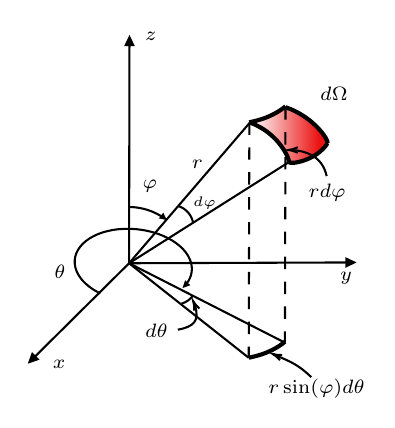
\begin{tikzpicture}[x=0.75pt,y=0.75pt,yscale=-1,xscale=1]
%uncomment if require: \path (0,300); %set diagram left start at 0, and has height of 300

%Shape: Polygon Curved [id:ds8617769563499198] 
\path  [shading=_0cl29xk28,_cudcahyu5] (309.66,113.18) .. controls (310.82,112.05) and (319.75,110.69) .. (323.46,106.69) .. controls (327.18,102.69) and (344.16,117.24) .. (345.31,122.38) .. controls (346.45,127.53) and (328.08,134.69) .. (326.76,132.29) .. controls (325.44,129.89) and (324.63,124.88) .. (321,121.31) .. controls (317.37,117.73) and (308.5,114.3) .. (309.66,113.18) -- cycle ; % for fading 
 \draw  [color={rgb, 255:red, 198; green, 2; blue, 2 }  ,draw opacity=1 ] (309.66,113.18) .. controls (310.82,112.05) and (319.75,110.69) .. (323.46,106.69) .. controls (327.18,102.69) and (344.16,117.24) .. (345.31,122.38) .. controls (346.45,127.53) and (328.08,134.69) .. (326.76,132.29) .. controls (325.44,129.89) and (324.63,124.88) .. (321,121.31) .. controls (317.37,117.73) and (308.5,114.3) .. (309.66,113.18) -- cycle ; % for border 

%Curve Lines [id:da7808313112872147] 
\draw [color={rgb, 255:red, 0; green, 0; blue, 0 }  ,draw opacity=1 ][line width=1.5]    (307.75,113.13) .. controls (321.25,117.63) and (327.44,130.74) .. (326.76,132.29) ;
%Curve Lines [id:da2280552545088137] 
\draw [color={rgb, 255:red, 0; green, 0; blue, 0 }  ,draw opacity=1 ][line width=1.5]    (325.17,105.82) .. controls (338.67,110.32) and (346.07,121.62) .. (345.4,123.17) ;
%Straight Lines [id:da24830770948666592] 
\draw    (249.99,74) -- (249.8,181) ;
\draw [shift={(250,71)}, rotate = 90.1] [fill={rgb, 255:red, 0; green, 0; blue, 0 }  ][line width=0.08]  [draw opacity=0] (5.36,-2.57) -- (0,0) -- (5.36,2.57) -- cycle    ;
%Straight Lines [id:da753659325232259] 
\draw    (356.4,180.61) -- (249.8,181) ;
\draw [shift={(359.4,180.6)}, rotate = 179.79] [fill={rgb, 255:red, 0; green, 0; blue, 0 }  ][line width=0.08]  [draw opacity=0] (5.36,-2.57) -- (0,0) -- (5.36,2.57) -- cycle    ;
%Straight Lines [id:da7343159766529195] 
\draw    (249.8,181) -- (203.13,227.29) ;
\draw [shift={(201,229.4)}, rotate = 315.24] [fill={rgb, 255:red, 0; green, 0; blue, 0 }  ][line width=0.08]  [draw opacity=0] (5.36,-2.57) -- (0,0) -- (5.36,2.57) -- cycle    ;
%Straight Lines [id:da38079896767960186] 
\draw    (249.8,181) -- (307.75,113.53) ;
%Straight Lines [id:da6137783505600632] 
\draw    (249.8,181) -- (326.76,132.29) ;
%Straight Lines [id:da41668418232759097] 
\draw  [dash pattern={on 4.5pt off 4.5pt}]  (307.75,113.13) -- (307.46,226.55) ;
%Straight Lines [id:da46125394152823274] 
\draw  [dash pattern={on 4.5pt off 4.5pt}]  (325.17,105.82) -- (324.88,219.25) ;
%Curve Lines [id:da8321014996922751] 
\draw [line width=1.5]    (326.76,132.29) .. controls (327.57,133.57) and (340.14,131.57) .. (345.4,123.17) ;
%Curve Lines [id:da6239818870261494] 
\draw [line width=1.5]    (307.75,113.13) .. controls (308.12,112.79) and (317.15,111.92) .. (325.17,105.42) ;
%Curve Lines [id:da5954080429412669] 
\draw [line width=1.5]    (307.46,226.55) .. controls (307.83,226.22) and (316.87,225.35) .. (324.88,218.85) ;
%Straight Lines [id:da2080670594856281] 
\draw    (249.8,181) -- (307.46,226.55) ;
%Straight Lines [id:da5162942524385837] 
\draw    (249.8,181) -- (324.88,219.25) ;
%Shape: Arc [id:dp12750654176978538] 
\draw  [draw opacity=0] (273.55,153.44) .. controls (277.36,154.66) and (280.08,157.93) .. (280.7,161.76) -- (270.37,163.41) -- cycle ; \draw   (273.55,153.44) .. controls (277.36,154.66) and (280.08,157.93) .. (280.7,161.76) ;  
%Shape: Arc [id:dp4429192150661687] 
\draw  [draw opacity=0] (280.42,196.83) .. controls (279.08,198.56) and (277.2,199.84) .. (275.07,200.46) -- (272.17,190.41) -- cycle ; \draw   (280.42,196.83) .. controls (279.08,198.56) and (277.2,199.84) .. (275.07,200.46) ;  
%Curve Lines [id:da9082322706507093] 
\draw    (273.29,213) .. controls (280.5,211.66) and (284.21,209.08) .. (281.4,201.04) ;
\draw [shift={(280.71,199.29)}, rotate = 67.01] [color={rgb, 255:red, 0; green, 0; blue, 0 }  ][line width=0.75]    (4.37,-1.32) .. controls (2.78,-0.56) and (1.32,-0.12) .. (0,0) .. controls (1.32,0.12) and (2.78,0.56) .. (4.37,1.32)   ;
%Shape: Arc [id:dp3505060548713421] 
\draw  [draw opacity=0] (250.06,153.9) .. controls (254.62,153.96) and (259.23,155.07) .. (263.54,157.33) .. controls (265.15,158.17) and (266.64,159.14) .. (268.03,160.21) -- (249.61,183.9) -- cycle ; \draw    (250.06,153.9) .. controls (254.62,153.96) and (259.23,155.07) .. (263.54,157.33) .. controls (264.24,157.7) and (264.92,158.09) .. (265.58,158.5) ; \draw [shift={(268.03,160.21)}, rotate = 217.79] [fill={rgb, 255:red, 0; green, 0; blue, 0 }  ][line width=0.08]  [draw opacity=0] (3.57,-1.72) -- (0,0) -- (3.57,1.72) -- cycle    ; 
%Shape: Arc [id:dp5681499560456225] 
\draw  [draw opacity=0] (235.91,195.52) .. controls (230.46,192.88) and (226.27,189.13) .. (224.49,184.74) .. controls (220.58,175.13) and (229.64,166.11) .. (244.73,164.6) .. controls (259.82,163.09) and (275.23,169.66) .. (279.14,179.27) .. controls (281.2,184.33) and (279.67,189.22) .. (275.55,192.94) -- (251.81,182) -- cycle ; \draw    (235.91,195.52) .. controls (230.46,192.88) and (226.27,189.13) .. (224.49,184.74) .. controls (220.58,175.13) and (229.64,166.11) .. (244.73,164.6) .. controls (259.82,163.09) and (275.23,169.66) .. (279.14,179.27) .. controls (280.82,183.39) and (280.11,187.4) .. (277.56,190.76) ; \draw [shift={(275.55,192.94)}, rotate = 314.31] [fill={rgb, 255:red, 0; green, 0; blue, 0 }  ][line width=0.08]  [draw opacity=0] (3.57,-1.72) -- (0,0) -- (3.57,1.72) -- cycle    ; 
%Curve Lines [id:da7436988002902412] 
\draw    (345,139) .. controls (342.75,128.75) and (333.94,126.81) .. (328.71,126.49) ;
\draw [shift={(326.71,126.43)}, rotate = 360] [color={rgb, 255:red, 0; green, 0; blue, 0 }  ][line width=0.75]    (4.37,-1.32) .. controls (2.78,-0.56) and (1.32,-0.12) .. (0,0) .. controls (1.32,0.12) and (2.78,0.56) .. (4.37,1.32)   ;
%Curve Lines [id:da27139248127484605] 
\draw    (337.57,235.86) .. controls (331.46,230.01) and (328.07,228.61) .. (320.73,225.46) ;
\draw [shift={(319,224.71)}, rotate = 23.43] [color={rgb, 255:red, 0; green, 0; blue, 0 }  ][line width=0.75]    (4.37,-1.32) .. controls (2.78,-0.56) and (1.32,-0.12) .. (0,0) .. controls (1.32,0.12) and (2.78,0.56) .. (4.37,1.32)   ;

% Text Node
\draw (256,208.57) node [anchor=north west][inner sep=0.75pt]  [font=\scriptsize] [align=left] {$\displaystyle d\theta $};
% Text Node
\draw (254.86,139.29) node [anchor=north west][inner sep=0.75pt]  [font=\scriptsize] [align=left] {$\displaystyle \varphi $};
% Text Node
\draw (279.14,147.29) node [anchor=north west][inner sep=0.75pt]  [font=\tiny] [align=left] {$\displaystyle d\varphi $};
% Text Node
\draw (212.29,180.29) node [anchor=north west][inner sep=0.75pt]  [font=\scriptsize] [align=left] {$\displaystyle \theta $};
% Text Node
\draw (334.86,141.14) node [anchor=north west][inner sep=0.75pt]  [font=\scriptsize] [align=left] {$\displaystyle rd\varphi $};
% Text Node
\draw (278.57,130) node [anchor=north west][inner sep=0.75pt]  [font=\scriptsize] [align=left] {$\displaystyle r$};
% Text Node
\draw (315.46,235.17) node [anchor=north west][inner sep=0.75pt]  [font=\scriptsize] [align=left] {$\displaystyle r\sin( \varphi ) d\theta $};
% Text Node
\draw (211.6,226.4) node [anchor=north west][inner sep=0.75pt]  [font=\scriptsize] [align=left] {$\displaystyle x$};
% Text Node
\draw (256,68) node [anchor=north west][inner sep=0.75pt]  [font=\scriptsize] [align=left] {$\displaystyle z$};
% Text Node
\draw (350,183.6) node [anchor=north west][inner sep=0.75pt]  [font=\scriptsize] [align=left] {$\displaystyle y$};
% Text Node
\draw (340.4,94.6) node [anchor=north west][inner sep=0.75pt]  [font=\scriptsize] [align=left] {$\displaystyle d\Omega$};


\end{tikzpicture}
